\documentclass{standalone}
	\usepackage{tikz}
		\graphicspath{ {figures/AM_10_463/} }
	\begin{document}
\begin{tikzpicture}[node distance=0.01cm and 3cm]
 \node[anchor=center] (0) at (0,-0.8) { 10 \ (block4\_conv3) };
\node[anchor=center] at (6,-0.8) { 11 \ (block5\_conv1) };
 \foreach \label [count=\i] in {L9_F247.png,L9_F205.png,L9_F444.png,L9_F432.png,L9_F125.png,L9_F413.png,L9_F59.png,L9_F250.png,L9_F21.png,L9_F208.png,L9_F40.png,L9_F434.png,L9_F88.png,L9_F443.png,L9_F426.png,L9_F467.png,L9_F359.png,L9_F222.png} { 
 
	\node[draw=none] (\i) at (0,-\i*6em) {\includegraphics[width=0.3\textwidth]{\label} }; 
  }
\node[] (R) at (6,-9.5*6em) {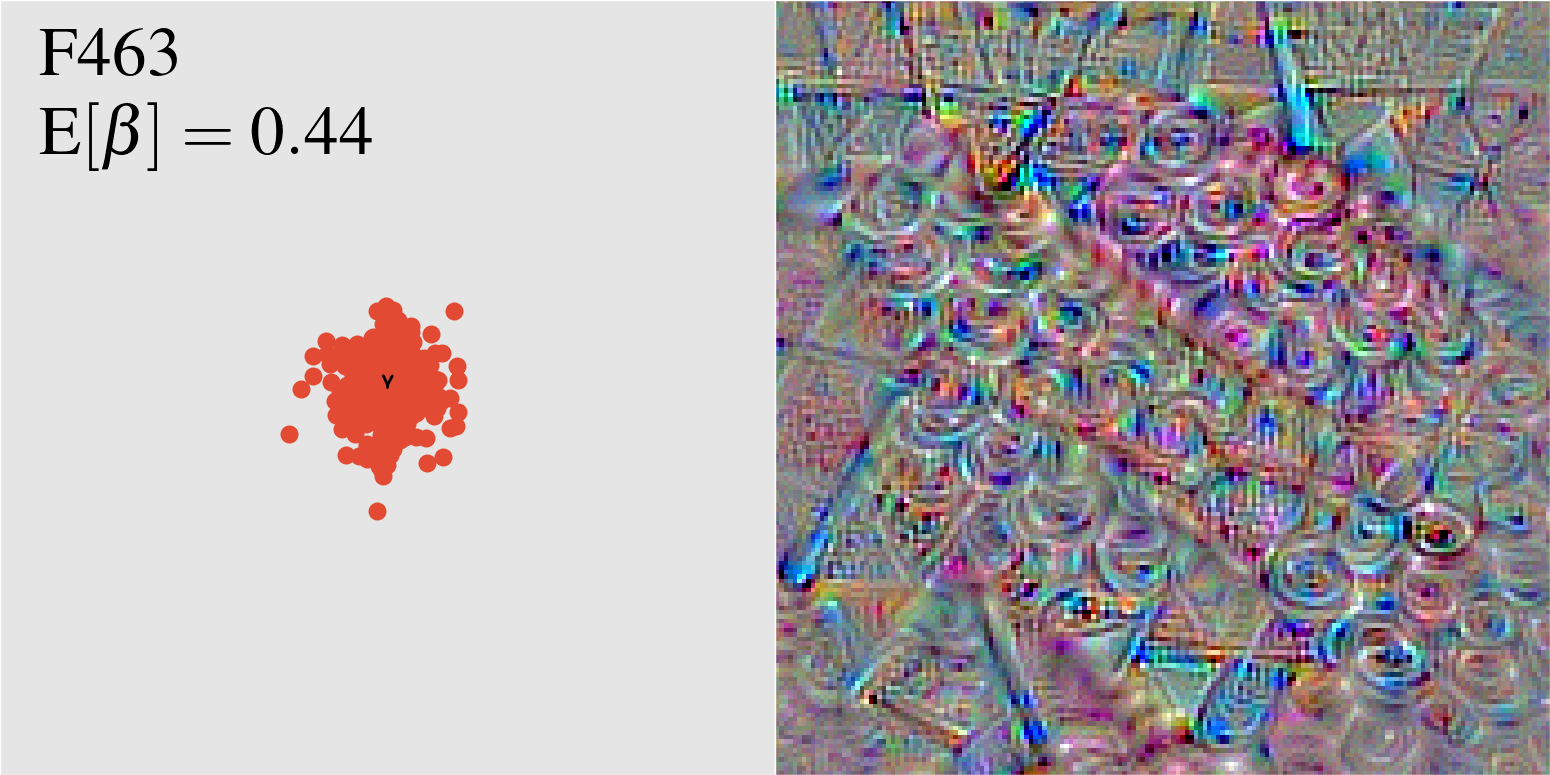
\includegraphics[width=0.3\textwidth]{ L10_F463.png } }; % Adjust the y-coordinate to center
 \draw (1.east) -- (R) node[pos=0.5, circle, draw, fill=white, minimum size=8pt, inner sep=0pt, scale=0.8] {$-$}; 
 \draw (2.east) -- (R) node[pos=0.5, circle, draw, fill=white, minimum size=8pt, inner sep=0pt, scale=0.8] {$-$}; 
 \draw (3.east) -- (R) node[pos=0.5, circle, draw, fill=white, minimum size=8pt, inner sep=0pt, scale=0.8] {$-$}; 
 \draw (4.east) -- (R) node[pos=0.5, circle, draw, fill=white, minimum size=8pt, inner sep=0pt, scale=0.8] {$-$}; 
 \draw (5.east) -- (R) node[pos=0.5, circle, draw, fill=white, minimum size=8pt, inner sep=0pt, scale=0.8] {$-$}; 
 \draw (6.east) -- (R) node[pos=0.5, circle, draw, fill=white, minimum size=8pt, inner sep=0pt, scale=0.8] {$-$}; 
 \draw (7.east) -- (R) node[pos=0.5, circle, draw, fill=white, minimum size=8pt, inner sep=0pt, scale=0.8] {$-$}; 
 \draw (8.east) -- (R) node[pos=0.5, circle, draw, fill=white, minimum size=8pt, inner sep=0pt, scale=0.8] {$-$}; 
 \draw (9.east) -- (R) node[pos=0.5, circle, draw, fill=white, minimum size=8pt, inner sep=0pt, scale=0.8] {$-$}; 
 \draw (10.east) -- (R) node[pos=0.5, circle, draw, fill=white, minimum size=8pt, inner sep=0pt, scale=0.8] {$-$}; 
 \draw (11.east) -- (R) node[pos=0.5, circle, draw, fill=white, minimum size=8pt, inner sep=0pt, scale=0.8] {$-$}; 
 \draw (12.east) -- (R) node[pos=0.5, circle, draw, fill=white, minimum size=8pt, inner sep=0pt, scale=0.8] {$-$}; 
 \draw (13.east) -- (R) node[pos=0.5, circle, draw, fill=white, minimum size=8pt, inner sep=0pt, scale=0.8] {$-$}; 
 \draw (14.east) -- (R) node[pos=0.5, circle, draw, fill=white, minimum size=8pt, inner sep=0pt, scale=0.8] {$-$}; 
 \draw (15.east) -- (R) node[pos=0.5, circle, draw, fill=white, minimum size=8pt, inner sep=0pt, scale=0.5] { 0.0 }; 
 \draw (16.east) -- (R) node[pos=0.5, circle, draw, fill=white, minimum size=8pt, inner sep=0pt, scale=0.5] { -1.0 }; 
 \draw (17.east) -- (R) node[pos=0.5, circle, draw, fill=white, minimum size=8pt, inner sep=0pt, scale=0.8] {$+$}; 
 \draw (18.east) -- (R) node[pos=0.5, circle, draw, fill=white, minimum size=8pt, inner sep=0pt, scale=0.8] {$+$}; 
\end{tikzpicture}
\end{document}
